\documentclass[aspectratio=169,english]{beamer}

% a opção hideSubsectionTitle esconde o título das subseções
\usepackage{templateLIPES}      % o arquivo templateLIPES.sty possui todo o estilo de formatação
\usepackage[portuguese]{babel}     % mude o idioma, caso necessite
\usepackage[alf, abnt-emphasize=bf, abnt-etal-text=it]{abntex2cite}

\setbeamertemplate{bibliography item}{}
\renewcommand{\theenumiv}{}

\begin{document}

\titulo{Incorporación de técnicas de muestreo mediante histogramas multidimensionales al código de simulación de fuentes de Monte Carlo KDSource}
% \subtitulo{Subtítulo}       % caso não haja, comente

\autor{Lucas Ezequiel Ovando}
\orientador{Dr. Ariel Marquez}        % caso não haja, comente
\coorientador{Ing. Zoe Prieto}      % caso não haja, comente

\curso{Ingenieria Nuclear}

\local{San Carlos de Bariloche, Rio Negro, Argentina}
\dia{12}
\mes{Febrero}
\ano{2025}

% NÃO REMOVA!
\begin{frame}[plain]
    
    \begin{tikzpicture}[overlay,remember picture]
        \node[left=-0.15cm] at (current page.0){
            \includegraphics[scale=0.145]{imagens/capaLIPES}
        };
    \end{tikzpicture}

    \titlepage
    
\end{frame}

\section[Outline]{}

\begin{frame}[allowframebreaks]
    \frametitle{Outline}
    \tableofcontents
\end{frame}

% CONTEÚDO -----------------------------------------------------------------

\section{Introdução}
\begin{frame}{Introdução}
    \begin{itemize}
        \item Teste 1
        \item Teste 2
        \item Teste 3
    \end{itemize}
\end{frame}

\section{Figura}
\begin{frame}{Figura}
    \begin{figure}
        \centering
        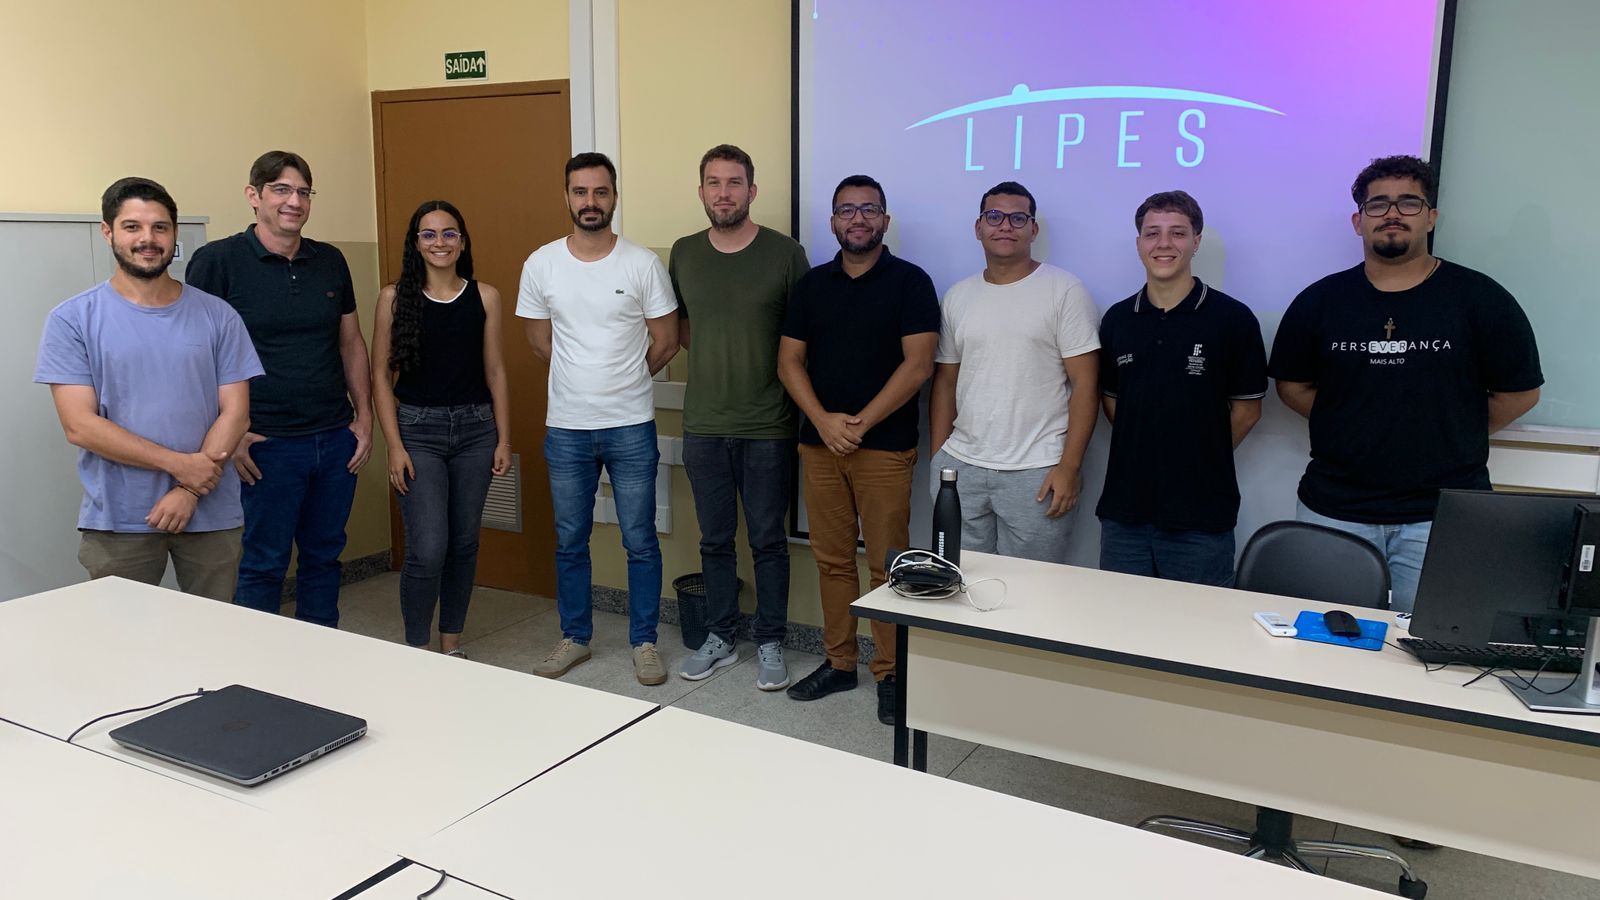
\includegraphics[width=0.6\linewidth]{imagens/1_seminario_LIPES.jpeg}
        \caption{1º seminário do LIPES em 27/01/2025}
        \label{fig:1semlipes}
    \end{figure}
\end{frame}

\section{Código}
\begin{frame}[fragile]{Código}
\begin{minted}{python}
from qiskit import QuantumRegister, QuantumCircuit
from numpy import pi

qreg_q = QuantumRegister(2, 'q')
circuit = QuantumCircuit(qreg_q)

circuit.h(qreg_q[0])
circuit.cx(qreg_q[0], qreg_q[1])
\end{minted}
\end{frame}

\section{Citação}
\begin{frame}{Citação}
    \begin{itemize}
        \item De acordo com \citeonline{fernandes2017} ...
        \item ... lorem ipsum \cite{fernandes2023}.
    \end{itemize}
\end{frame}

% FIM DO CONTEÚDO -----------------------------------------------------------------

% NÃO REMOVA!
\section{Referências}
\begin{frame}[allowframebreaks]
    \addtocounter{framenumber}{-1}
    \frametitle{Referências}
    \scriptsize
    % \bibliographystyle{abntex2-alf-en}  % mude para qualquer arquivo .bst
    \bibliography{referencias}
\end{frame}     
\end{document}